\documentclass[man, noapacite, 12pt]{apa2}

\makeatletter
\newenvironment{chapquote}[2][2em]
  {\setlength{\@tempdima}{#1}%
   \def\chapquote@author{#2}%
   \parshape 1 \@tempdima \dimexpr\textwidth-2\@tempdima\relax%
   \itshape}
  {\par\normalfont\hfill--\ \chapquote@author\hspace*{\@tempdima}\par\bigskip}
\makeatother

%\usepackage{pdfsync}
\usepackage{amsmath}
\usepackage{graphicx}
%\usepackage{topcapt}
%\usepackage{color}
%\usepackage{comment}
\usepackage{booktabs}
\usepackage{apacite2}
\usepackage{fullpage,rotating}
\usepackage{pslatex}
\usepackage{amssymb}
\usepackage{multirow}


\title{Linguistic structure emerges from cognitive mechanisms}
\author{Molly L. Lewis}
\affiliation{Department of Psychology, Stanford University\\ Conceptual Analysis of Dissertation Area\\ 6 October 2014}


\shorttitle{Linguistic structure emerges from cognitive mechanisms}
\rightheader{Linguistic structure emerges from cognitive mechanisms}
\acknowledgements{Advisor: Michael C. Frank\\ \noindent Additional Readers: Ellen Markman and Noah Goodman}

\abstract{People interact with people and, because of shared interest, try to coordinate their behavior. This behavior is governed by the competition of pragmatic pressures. These pressures lead to equilibria. These equilibria become conventionalized over time (Lewis). This convention becomes an additional pressure in the moment of interaction. Language as a paradigm case of these dynamics.}

\begin{document}
\maketitle

%%%%%%%%% INTRO %%%%%%%%% 
%\begin{chapquote}{Aristotle, \textit{Nic. Ethics II 6}}
%\noindent  Virtue, then, is a state of character concerned with choice, lying in a mean, i.e. the mean relative to us, this being determined by a rational principle, and by that principle by which the man of practical wisdom would determine it. Now it is a mean between two vices, that which depends on excess and that which depends on defect; and again it is a mean because the vices respectively fall short of or exceed what is right in both passions and actions, while virtue both finds and chooses that which is intermediate. Hence in respect of its substance and the definition which states its essence virtue is a mean, with regard to what is best and right an extreme.
%\end{chapquote}

\begin{chapquote}{G.K. Zipf, \textit{1949}}
\noindent  Human society can be viewed as a field which both influences the individual members of the group and is influenced by them. 
\end{chapquote}

\section{Introduction}
``Room for cream?'' asked the barista. ``Mm, yes -- just a bit" replied the customer. Mundane linguistic interactions such as this are the building blocks of daily experience. They are individuals making sounds to each other in an effort to coordinate their behavior in the physical world \cite{clark2006social}. These interactions are messy, variable, and highly unconstrained. Indeed it is this variability that gives language its vast expressive power \cite{hockett1960}. Yet, despite this appearance of irregularity, rich patterns in linguistic usage are revealed when we aggregate across instances of language use both within and across languages. At the level of syntax, for example, there is a strong bias in English to put subjects before verbs and, across languages, this pattern is attested more often than would be expected by chance alone  \cite{dryer2005order}. These types of probabilistic regularities exist at every level of linguistic structure --- from phonology, to semantics, syntax, and discourse --- and researchers from a variety of disciplines have taken as their project the goal of characterizing these regularities.

In this paper, I argue that we can gain  insight into the character of linguistic structure by considering the dynamics of language use. I will suggest the best way to do this is by framing language use as an instance of a broader phenomenon: social interaction \cite{clark1996using}. In particular, I will adopt the formal framework of social interaction proposed by Thomas Schelling, in which social interactions are viewed as acts of solving coordination problems.  To illustrate, consider the barista example above. In this example, the agents are the barista and the customer, and they must coordinate how  to fill the coffee mug. There are two outcomes --- full and almost full --- and the barista's desired outcome is determined by the preference of the customer. In this case, the barista and the customer rely on language to coordinate their behavior, but this coordination could have been achieved in other ways (e.g. the customer could have shook her head, pointed to the place inside the mug that she wanted the coffee filled to, etc.). Coordination of their behavior is achieved  by arriving at the mutually preferred outcome (the customer's mug is almost full).

A key tenet to the broader argument is that the act of using language is itself an act of solving a coordination problem \cite{clark1996using}. When a person speaks, there are many possible ways the utterance could be interpreted, and arriving at the intended interpretation is an act of coordination. For example, in the case of the customer's interaction with the barista, there are many possible interpretations of the phrase, ``Room for cream?." The barista could mean ``Would you like to add cream to your coffee? If so, I will facilitate that by not filling your mug full with coffee." Or, ``We have so much extra inventory of cream! Do you have room in your bag to take some?" Or, ``Do you like the band `Room for cream'?". Or, if the speaker is speaking another language, a totally unrelated meaning. The point is that the speaker's intended meaning is underspecified from the language alone and the interlocutors must work collaboratively to arrive at a shared understanding. Following \citeA{lewis1969convention}, I will suggest that we can gain insight into the dynamics of linguistic coordination problems such as this by using Schelling's formal framework.  This perspective on language use will ultimately provide a helpful framework for understanding the relationship between language use and language structure.

In Part I, I will outline the linguistic coordination problem as a paradigmatic case of the social coordination problem. I will suggest that coordination problems are solved through the dynamics of two opposing two forces --- the goals of the one's self and the goal of the other. Following Lewis, I suggest that these opposing forces are resolved by finding an equilibrium point. I will then argue that the equilibria that are reached in language use are reflected in the structure of language, and survey a variety of phenomena in linguistic structure that show this pattern.

In Part II, I will consider the mechanism that might cause linguistic structure to reflect the equilibria reached in linguistic use. Lewis argued that once individuals succeed in solving a coordination problem, there is a tendency to stick with that solution (even though other, equally good solutions exist). This solution is called a convention. I will argue that the key to understanding the link between regularities in linguistic usage and linguistic structure is the process of children's acquisition of these conventions. I will consider how the dynamics of language acquisition might lead to language change. Finally, I will consider the complementary role of conventions and cognitive forces in solving language coordination problems, and the  empirical challenge associated with disentangling the two.

%%%%%%%%% PART I %%%%%%%%% 
\section{Part I: Linguistic structure reflects pragmatic equilibria}

Where does linguistic structure come from? \citeA[2010]{christiansen2008} propose a compelling theory. They argue that  multiple cognitive constraints dynamicaly influence language evolution. They suggest four constraints: the representational format of thought, properties of the percepto-motor system, learning and processing constraints, and so-called `pragmatic' constraints. Pragmatic constraints are the result of reasoning about another speaker's intention in context. Their argument is that these  cognitive constraints  influence  language at the moment of use, but over time, these biases become instantiated in the structure of language. Although each of these constraints likely plays an important role in the evolution of language, the present paper focuses on the independent contribution of pragmatic constraints. The claim is that in-the-moment pragmatic constraints become fossilized in the structure of language over time. To develop this claim, we begin by modeling language use as a type of social coordination.

\subsection{Social interaction as a coordination problem}
The idea that language is an instance of a much broader class of behavioral phenomenon --- social coordination --- has been noted by many theorist of language \cite{zipf1936, lewis1969convention, grice1975logic, clark1996using}. Each viewed language use as a case of multiple agents making interdependent  rational choices.\footnote{In outlining his seminal theory of pragmatics, Grice  writes: ``As one of my avowed aims is to see talking as a special case or variety of purposive, indeed rational, behaviour, it may be worth noting that the specific expectations of presumptions connected with at least some of the foregoing maxims have their analogues in the sphere of transactions that are not talk exchanges" \cite[pg. 47]{grice1975logic}.} Nonetheless, language use is a paradigmatic case of a coordination problem: it provides a tool that is universal in a community, easy to use, and capable of expressing complex ideas.

\citeA{lewis1969convention} formalized the notion of language as a coordination problem by adopting work from game theory. He defines a  {\it coordination problem} as follows: \begin{quote} Two or more agents must each choose one of several alternative actions. Often all the agents have the same set of alternative actions, but that is not necessary. The outcomes the agents want to produce or prevent are determined jointly by the actions of all the agents (p. 8).
\end{quote} 
The key feature of these problems is that some combinations of the agents' choices are better than others: there are a set of equilibria of joint choices in which no agent would have a larger payoff had the agent alone changed their choice.

This broad framing can describe the dynamics of many social interactions. Take the above case of the barista and the customer, for example. We can model this interaction using a payoff matrix (Table 1). In the matrix, we represent the customer's payoff along the rows and the barista's payoff along the columns. There are two possible choices for  level of coffee in the cup---  full and  almost full --- and so each agent gets two rows or columns. 
\begin{table}[t]
\begin{center}
\begin{tabular}{l p{3cm} l p{3cm} l p{3cm} l}
 &  & \multicolumn{2}{c}{customer} \\ \cline{2-4} 
\multicolumn{1}{l|}{} & \multicolumn{1}{l|}{} & \multicolumn{1}{l|}{full} & \multicolumn{1}{l|}{almost full} \\ \cline{2-4} 
\multicolumn{1}{c|}{\multirow{2}{*}{barista}} & \multicolumn{1}{l|}{full} & \multicolumn{1}{l|}{0,0} & \multicolumn{1}{l|}{0,0} \\ \cline{2-4} 
\multicolumn{1}{c|}{} & \multicolumn{1}{l|}{almost full} & \multicolumn{1}{l|}{0,0} & \multicolumn{1}{l|}{1,1} \\ \cline{2-4} 
\end{tabular}
\caption{}
\end{center}
\end{table}
The agents relative payoffs are indicated in the cells, with the barista's on the left, and the customer's on the right. This happens to be a very simple equilibria --- there is one, and only one, possible set of actions in which is an equilibrium. The customer prefers almost full and the barista fills the cup to almost full. The problem is that the barista does not know a priori where this equilibrium lies, i.e. that the customer's pay off for almost full is 1, relative to 0 for full. To solve this coordination problem, the customer and barista make use of language.

More complicated coordination problems arise when there are multiple possible equilibria. Consider a weekend trip in which food and alcohol must be brought. To distribute the burden, half of the vacationers will bring food and the other half alcohol. In this case, the pay off matrix might look something like Table 2. Neither group --- Group A or B --- has a strong preference about which of the two commodities they bring. However, what is important is that one group brings food and the other alcohol (no one will be happy on a weekend trip with only food or only alcohol). There are thus two equilibria, one each at a  set of choices where the two groups bring different things. By chance, the vacationers are equally likely to end up in a non-equilibrium as they are an equilibria. They must  therefore coordinate, via language or some other means, to ensure that they end up in an equilibrium.

\begin{table}[t]
\begin{center}
\begin{tabular}{l p{3cm} l p{3cm} l p{3cm} l}
 &  & \multicolumn{2}{c}{Group A} \\ \cline{2-4} 
\multicolumn{1}{l|}{} & \multicolumn{1}{l|}{} & \multicolumn{1}{l|}{food} & \multicolumn{1}{l|}{alcohol} \\ \cline{2-4} 
\multicolumn{1}{c|}{\multirow{2}{*}{Group B}} & \multicolumn{1}{l|}{food} & \multicolumn{1}{l|}{0,0} & \multicolumn{1}{l|}{1,1} \\ \cline{2-4} 
\multicolumn{1}{c|}{} & \multicolumn{1}{l|}{alcohol} & \multicolumn{1}{l|}{1,1} & \multicolumn{1}{l|}{0,0} \\ \cline{2-4} 
\end{tabular}
\caption{}
\end{center}
\end{table}

What are the psychological forces that support these coordination games? Zipf suggested a parsimonious way to think about the psychological forces at play in these interactions. He suggested that all equilibria could provided  lead to the resolution of an equilibrium point in a coordination game. Zipf argued that dynamical systems were the result a single force.

Examples beyond economics

\subsection{Language use as a coordination problem}

The coordination problem framework can be straight-forwardly applied to language use \cite{lewis1969convention}. In the case of language use, the coordination problem lies in the resolution of reference. Broadly,  resolving reference requires interpreting a meaning from some linguistic form. This is a difficult problem because the relationship between linguistic form and meaning is arbitrary \cite{saussure, hockett1960}. That is, knowing the form of a word does not give a language user any insight into the meaning of that word. Consequently, because there is no inherent mapping between form and meaning, speakers must coordinate their behavior. 

\begin{table}[t]
\begin{center}
\begin{tabular}{l p{3cm} l p{3cm} l p{3cm} l}
 &  & \multicolumn{2}{c}{Speaker 1} \\ \cline{2-4} 
\multicolumn{1}{l|}{} & \multicolumn{1}{l|}{} & \multicolumn{1}{l|}{``fep"} & \multicolumn{1}{l|}{``dax"} \\ \cline{2-4} 
\multicolumn{1}{c|}{\multirow{2}{*}{Speaker 2}} & \multicolumn{1}{l|}{Object A} & \multicolumn{1}{l|}{0,0} & \multicolumn{1}{l|}{1,1} \\ \cline{2-4} 
\multicolumn{1}{c|}{} & \multicolumn{1}{l|}{Object B} & \multicolumn{1}{l|}{1,1} & \multicolumn{1}{l|}{0,0} \\ \cline{2-4} 
\end{tabular}
\caption{}
\end{center}
\end{table}

The arbitrariness of linguistic form leads to a formal equivalence between the problem of reference and the problems of coordination described above.  To understand this similarity, consider the a case where someone there are two novel words,``dax" and ``fep," and two novel objects, Object A and Object B. Given this information alone, the listener has no a priori insight into which object each word refers to. This is a problem because the two interlocutors must somehow arrive at the same mappings between words and referents in order to communication (a system in which you call Object A ``fep" and I call it ``dax" is a terrible communication system). The interlocutors must therefore coordinate. 

The payoff structure of this problem looks just like the vacationer example above (Table 3). Because language is arbitrary, neither speaker cares whether you call Object A ``fep" or ``dax;" they only care that their mappings are the same.  These general dynamics are true not only of individual lexical items, but of all cases of reference. Consider again our example of the barista and the customer. In interpreting the phrase, ``Room for cream?,"the individual lexical items are relatively unambiguous --- presumably both know what ``room" and ``cream" mean. But, the intended meaning of the entire phrase is underspecified, and so the interlocutors must work together to resolve meaning.

In this framework, we can think of {\it pragmatics} as the study of the psychological processes that lead to an equilibrium in these referential coordination problems. There have been numerous proposed taxonomies of xxx
Involved discussion of Horn 

This fits with the empirical data (one-shot reference problems)
\cite{frank2012predicting}, 


\subsection{Pragmatic equilibria reflected in the structure of language}
Consider four cases in which equilibrium points predicted by Horn's theory of pragmatics are reflected in the structure of language: lexicon, semantics, semantics and words.

\subsubsection{Lexicon}
\subsubsection{Semantics}
\subsubsection{Words}
\subsubsection{Syntax}

%%%%%%%%% PART II %%%%%%%%% 
\section{Part II: Understanding the mechanism leading to the similarity between the timescales}
Why does language structure reflect the patterns that appear in language use? In the present, section I propose a speculative answer to this question. Critically, the answer relies on an analysis of language separated by timescales. The hypothesis is that the reason structure reflects pragmatics is the result of local dynamics between each timescale and it's adjacent once

%%% Prag and discourse %% 
\subsection{the relationship between pragmatic and discourse} 
* Lewis- convention (

* Conceptual pacts
Framing  language use as a special case of conformity suggests that language use should be studied in a social context. There is evidence that speakers coordinate their linguistic behavior both in the language used to refer to a particular referent and the use of grammatical structures .  

Coordination of reference was demonstrated in an experimental task by \citeA{clark1986referring}. In this task, pairs of naive subjects were brought into the lab and randomly assigned to either the role of director or matcher. They were seated across from each other with an opaque wall in between them. Each subject had a set of 12 cards with ambiguous images (an identical set of 12 as their partner). The director had their 12 cards arranged in a 6-by-2 grid, and her task was to direct the matcher to organize her cards in the same way using only verbal instruction. They were allowed to interact as much as they desired. After repeatedly completing this task with the same partner, it was found that directors used overall fewer words to describe the cards over successive trials. This was achieved through developing shared conceptualizations of different cards. For example, in trial 1, one director used the phrase ``the next one looks like a person who's ice skating, except they're sticking their arms out in front", but by trial 6 the same director simply used the phrase ``the ice skater" to refer to that same card. This pattern suggests that interlocutors coordinate how they conceptualize the world through language, and this coordination increases over time.

Pacts in linguistics structure. Similar patterns have been observed in the coordination of linguistic structure. In a study by \citeA{branigan2000syntactic}, participants completed a picture description task in pairs. They alternated using a single sentence to describe the event depicted on different cards. Critically, one of the participants was a confederate. Sometimes the confederate used a prepositional object structure (e.g.\ ``The girl is throwing the ball to the dog.") and sometimes she used a double-object construction (e.g.\ ``The girl is throwing the dog the ball.").  The results revealed that subjects tended to use the syntactic structure used by the confederate to describe their own picture (even though there was no semantic overlap between the two). This result suggests that, within conversations, speakers may not only conform in how they conceptualize the world but also in the grammatical structures they use.

\cite{scott2009signalling}
daniel mathews (kids), metzing %& brennan , susan brenant

What are the psychological process supporting this behavior? When language use is couched in the context of the broader phenomenon of social interaction, old studies of social interaction become relevant. 

There is evidence for this emergent view of conformity from the original \citeA{sherif1935} study. In one version of the study, a group of three subjects were first tested individually in the light movement task. They were then tested three  additional times as a group. The group context was identical to the individual paradigm except that other subjects were also making judgements about the movement of the light at the same time. As in the Asch studies, subjects did not know each other prior to the experiment. Figure 1a plots the results of one group of three subjects. When tested individually, the three subjects were highly variable in their distance judgements. However, when tested together, their judgements tended to converge, and this convergence increased over iterations of the experiment. The inverse of this experiment was also conducted, in which subjects were first tested in a group and then individually. In this design, subjects showed conformity when tested together, and some divergence from the social norm once tested individually. Critically, however, they showed much less variability in the individual test in this design, as compared to the design in which they were tested individually first. This result provides additional evidence for the tendency of groups to converge at an (arbitrary) solution to a problem. In the case of linguistic meaning, this suggests that groups may arrive at shared (but theoretically arbitrary) ways of conceptualizing referents.

\begin{figure}
\begin{center} 
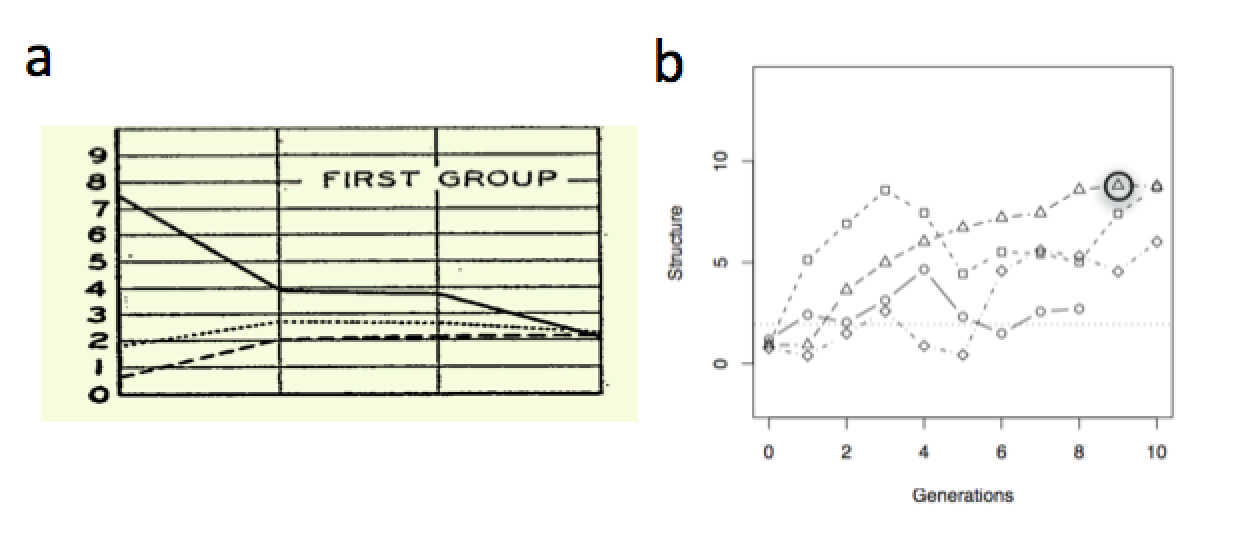
\includegraphics[width=5in]{figs/coordinatingmeaning.png}
\caption{\label{fig:results}  Plots reproduced from (a) Sherif (1935) and (b) Kirby,  Cornish, and Smith (2008). Plot (a) shows the median distance judgement (in inches) for three different subjects. The x-axis plots subjects performance on the task when completed individually, and then three subsequent periods in which the task was completed as a group (of 3 subjects).  Plot (b) shows the emergence of systematicity in the language across generations in the labeling task. Each line corresponds to a different set of people. Both plots suggest the emergence of systematicity, or conformity, within the group as a function of time. }
\end{center} 
\end{figure}

* unconcioncious, but increases with awareness

%%% Discourse and development %% 
\subsection{the relationship between discourse and development} 
*cached equilibrium, generalization problem, learning to learn, overhypothes

%%% Development and language %% 
\subsection{the relationship between development and linguistic structure}
- christiasen and chater

Recent work using an artificial language paradigm tests this prediction. In a study by \citeA{kirby2008cumulative}, participants were presented with a novel language and asked to learn the pairings between words to novel images. For the first subject, the mappings between words and images was randomly generated. In the training phase, the subject was presented with an image and a label for that image. In the testing phase, they were shown a new image and asked to guess what word they thought was associated with that image. This first subject's responses were recorded, then divided into half (one half for training and one half for testing), and presented to a subsequent subject. This process repeated for a total of 10 subjects. Consistent with the Sherif (1935) results, it was predicted that language use would become more systematic over time. In particular, it was predicted that a pattern should emerge in the mapping between features of the stimuli (e.g.\ color, shape, etc.) and syllables in the novel words. This is exactly what was found (Figure 1b). As the number of generations increased, the language became more systematic. This pattern was observed across a four different ``strings" of participants.

It suggests that the conformity that takes place in the context of particular conversations (as demonstrated by Brennan and Clark, 1996) has larger consequences when aggregated across time and across a linguistic community. While conversations are the locus of conformity,  many small instances of conformity lead to highly regularized language patterns at the level of linguistic communities.



\subsection{Two case studies: Me and refComplex}

\subsection{Consequences for learning}
Christiansen and Chater
�	Frank - Inferring word meaning by assuming speakers are informative
\cite{smith2013learning}
�	Ali�s adjective paper

\subsection{An empirical challenge: Sufficient but not necessary mechanisms}
Parallels between development and language structure, and development and pragmatics in the moment of language use


\bibliographystyle{apacite}
\bibliography{biblibrary}

\end{document}

